\begin{mainquestion}{circuit_graph}{Loops, Nodes, and Elements Oh My!}
Consider the following circuit diagram:

\begin{center}
    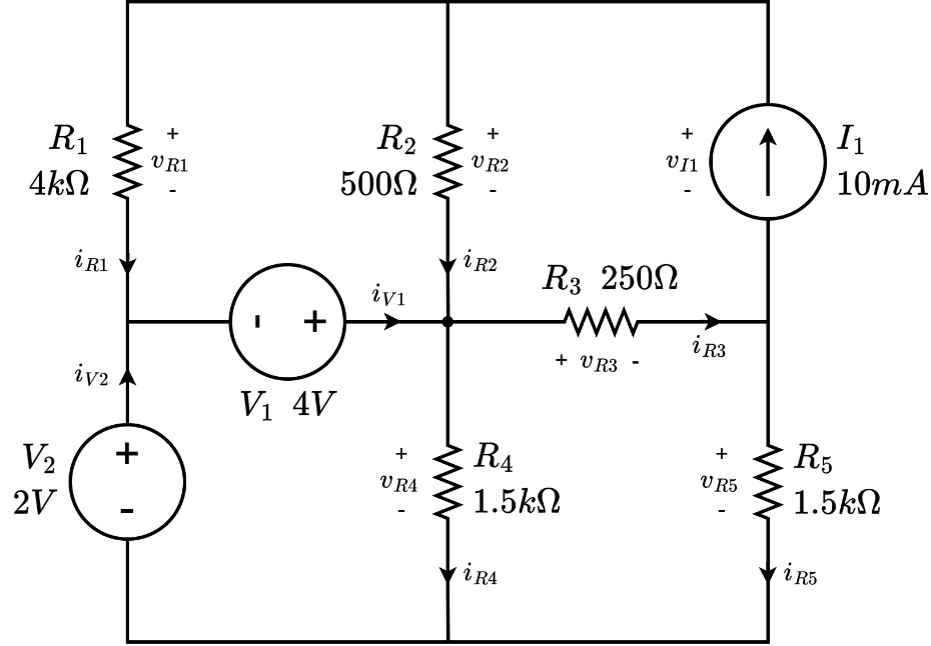
\includegraphics[]{schematic.png}
\end{center}

% =========================================================
\begin{partquestion}{nodes}
{How many nodes are in the circuit?}
\begin{answer}
    There are 5 nodes.
\end{answer}
\end{partquestion}

% =========================================================
\begin{partquestion}{loops}
{How many loops? How many independent loops?}
\begin{answer}
    There are 13 loops, although only 4 of them are independent.
\end{answer}
\end{partquestion}

% =========================================================
\begin{partquestion}{branches}
{How many branches?}
\begin{answer}
    There are 8 branches.  At this point, we can confirm the fundamental theorem of network topology:
    \begin{align*}
        b&=l+n-1\\
        &=4+5-1=8
    \end{align*}
\end{answer}
\end{partquestion}

% =========================================================
\begin{partquestion}{series}
{How many series elements are in the circuit?}
\begin{answer}
    There are no series elements in this circuit:  No two elements share a node exclusively.
\end{answer}
\end{partquestion}

% =========================================================
\begin{partquestion}{parallel}
{How many parallel elements are in the circuit?}
\begin{answer}
    There are no parallel elements in this circuit either!  No two elements share the same node at each of their respective terminals.
\end{answer}
\end{partquestion}

\end{mainquestion}